\documentclass[10pt]{beamer}

\usetheme[progressbar=frametitle]{metropolis}
\usepackage{appendixnumberbeamer}

\usepackage{booktabs}

% For removing Figure 1 in figures
\usepackage{caption}

% For enumeration as words
\usepackage{blindtext}
\usepackage{enumerate}
\usepackage{geometry}

\usepackage{tikz}
\usepackage{xspace}


\title{Theory of Computation}
\subtitle{Tutorial - Introduction to Grammars}
\author{Cesare Spinoso-Di Piano}
\date{}

\begin{document}

\maketitle

\begin{frame}{Plan for today}
    \setbeamertemplate{section in toc}[sections numbered]
    \tableofcontents[hideallsubsections]
\end{frame}

\section{What's a grammar?}

\begin{frame}{What's a grammar?}

\end{frame}

\section{Grammar formalization}

\begin{frame}{Definition}
    \textbf{Definition.} A grammar is a 4-tuple $G = (V, T, S, P)$ where
    \begin{itemize}
        \item $V$ is a finite set of variables (upper case symbols)
        \item $T$ is a finite set of terminals (lower case symbols)
        \item $S$ is the (unique) start variable
        \item $P$ is a finite set of productions
    \end{itemize}
    Productions in $P$ have the form $x \rightarrow y$ where, in their most general form, $x \in (T \cup V)^*$ and $y \in (T \cup V)^*$.
\end{frame}

\begin{frame}{Example}
    \textbf{Example.} $G = (V=\{S,A,B\},T=\{a,b\},S, P)$ where $P$ is
    \begin{align*}
        S & \rightarrow A|\lambda \\
        A & \rightarrow a|bbBa    \\
        B & \rightarrow b|\lambda
    \end{align*}
\end{frame}

\begin{frame}{Derivations}
    \textbf{Definition.} If using a sequence of productions we can obtain $y$ from $x$ we say $x$ \textbf{derives} $y$ or $x \Rightarrow^* y$.

    \textbf{Example.} From $G$ in the previous example,
    \begin{align*}
        S & \rightarrow A|\lambda \\
        A & \rightarrow a|bbBa    \\
        B & \rightarrow b|\lambda
    \end{align*}
    the grammar $G$ can generate the string $bbba$
    \begin{align*}
        S & \Rightarrow A \Rightarrow bbBa \Rightarrow bbba  \text{ or we can write it as }
        S \Rightarrow^* bbba
    \end{align*}
\end{frame}

\begin{frame}{Grammars as language generators}
    \textbf{Definition.} A grammar $G=(V,T,S,P)$ is said to \textbf{generate} a language $L(G)$ which is defined as $L(G) = \{w \in T^* : S \Rightarrow^* w\}$.

    \textbf{Example.} From $G$ in the previous example,
    \begin{align*}
        S & \rightarrow A|\lambda \\
        A & \rightarrow a|bbBa    \\
        B & \rightarrow b|\lambda
    \end{align*}
    we have
    \begin{itemize}
        \item $S \Rightarrow \lambda$
        \item $S \Rightarrow A \Rightarrow a$
        \item $S \Rightarrow A \Rightarrow bbBa \Rightarrow bba$
        \item $S \Rightarrow A \Rightarrow bbBa \Rightarrow bbba$
    \end{itemize}
    \begin{align*}
        L(G) & = \{\lambda, a, bba, bbba\}
    \end{align*}
\end{frame}

\begin{frame}{Exercise}
    \textbf{Exercise.} What is the language generated by the following grammar $G=(\{S,A,B\}, \{a,b\}, S, P)$ where $P$ is
    \begin{align*}
        S & \rightarrow Bb|\lambda  \\
        B & \rightarrow bbB|\lambda
    \end{align*}
    Starting with $S$ there are several possible derivations:
    \begin{itemize}
        \item Using the $\lambda$ derivation: $S \Rightarrow \lambda$

        \item Using the $Bb$ derivation:
              \begin{itemize}
                  \item $S \Rightarrow Bb \Rightarrow \lambda b = b $
                  \item $S \Rightarrow Bb \Rightarrow bbBb \Rightarrow bbb$
                  \item $S \Rightarrow Bb \Rightarrow bbBb \Rightarrow bbbbBb \Rightarrow bbbbb$
                  \item In general, $S \Rightarrow^* b(bb)^*$
              \end{itemize}
    \end{itemize}
    $L(G) = \{\lambda\} \cup \{b^{2n+1} : n \geq 0\}$
\end{frame}

\begin{frame}[t]{Exercise}
    \textbf{Exercise.} Determine $L(G)$ and \textit{prove} your answer. That is, if you claim that $L(G) = L$, show that this is the case. $G=(\{S\}, \{a,b\}, S, P)$ with $P$ as
    \begin{align*}
        S & \rightarrow aSb | aSbb | \lambda
    \end{align*}

\end{frame}

\section{Types of grammars}

\begin{frame}{Types of grammars}
    The type of a grammar is determined by the form its production rules can take on.
    \begin{enumerate}[1.]
        \item Left-linear and right-linear grammars
        \item Context-free grammars
        \item Context-sensitive grammars
        \item Unrestricted grammars
    \end{enumerate}
\end{frame}

\section{Regular grammars}

\begin{frame}{Left-linear grammars}
    % Definition plus example
    \textbf{Definition.} A grammar $G = (V,T,S,P)$ is \textbf{left-linear} if \underline{each} of the production rules in $P$ have one of the following forms:
    \begin{align*}
        A & \rightarrow Bx \\
        A & \rightarrow x
    \end{align*}
    Where $A,B \in V$ and $x \in T^*$. Can you give a slightly more formal definition?

    \textbf{Example.} The following is a left-linear grammar. What does it generate?
    \begin{align*}
        S & \rightarrow Aa | \lambda \\
        A & \rightarrow Sb           \\
    \end{align*}
\end{frame}

\begin{frame}{Right-linear grammars}
    \textbf{Definition.} A grammar $G = (V,T,S,P)$ is \textbf{right-linear} if \underline{each} of the production rules in $P$ have either of the following forms:
    \begin{align*}
        A & \rightarrow xB \\
        A & \rightarrow x
    \end{align*}
    Where $A,B \in V$ and $x \in T^*$.\\

    \textbf{Example.} The following is a right-linear grammar. What does it generate?
    \begin{align*}
        S & \rightarrow aA | \lambda \\
        A & \rightarrow bS           \\
    \end{align*}
\end{frame}

\begin{frame}{Regular grammars}
    \textbf{Definition.} A grammar $G$ is \textbf{regular} if it is either right-linear or left-linear.

    \textbf{Example.} Is the following grammar left-linear? Right-linear? Regular?
    \begin{align*}
        S & \rightarrow aaaA | \lambda \\
        A & \rightarrow abA | \lambda  \\
    \end{align*}
\end{frame}

\begin{frame}{Example}
    \textbf{Example.} Consider the grammar $G = \{V = \{S,A\}, T = \{a,b\}, S, P\}$ where $P$ is
    \begin{align*}
        S & \rightarrow aS|bS|abA     \\
        A & \rightarrow aA|bA|\lambda
    \end{align*}
    $G$ is a right-linear (and hence a regular) language.\\\bigskip
    Any string of the form $w_1abw_2, w_1,w_2 \in \{a,b\}^*$ can be generated by $G$. Suppose $w_1 = ba$, $w_2 = aa$:
    \begin{align*}
        S \Rightarrow bS \Rightarrow  baS \Rightarrow ba\textcolor{red}{ab}A \Rightarrow baabaA \Rightarrow baabaa
    \end{align*}
    $G$ generates $L(G) = \{w \in \{a,b\}^*: \text{ w contains $ab$ as a substring }\}$.
\end{frame}

\begin{frame}[t]{Exercise}
    \textbf{Exercise.} Write a regular grammar that generates $L = \{w \in \{a,b\}^*: |w| \mod 2 = 0\}$
\end{frame}

\section{Linear grammars}

\begin{frame}{Linear grammars}
    \textbf{Definition.} A grammar $G = (V,T,S,P)$ is linear if each of the production rules have the form $x \rightarrow y$ where $x \in V$ and $y \in T^* \cdot (V \cup \{\lambda\}) \cdot T^*$.

    \textbf{Example.} The following is a linear grammar. What does it generate?
    \begin{align*}
        S & \rightarrow aA | \lambda \\
        A & \rightarrow Sb           \\
    \end{align*}

    \textbf{Exercise.} Are all linear grammars also regular? Are all regular grammars also linear?
\end{frame}

\section{Regular grammars and regular languages}

\begin{frame}{Converting an FA to a right-linear grammar}
    Let $M = (Q, \Sigma, \delta, q_0, F)$ be an FA (either an NFA or a DFA). We want to create a right-linear grammar $G = (V, T, S, P)$ such that $L(G) = L(M)$. Let $V = Q, T = \Sigma, S = q_0$. Construct the production rules as follows:
    \begin{enumerate}[1.]
        \item For transitions of the form $\delta(q_i,\sigma)=q_j$, where $\sigma\in\Sigma$, create a production rule $q_i \rightarrow \sigma q_j$
        \item For transitions like $\delta(q_i,\lambda)=q_j$, create a production rule $q_i \rightarrow q_j$
        \item Create a production rule $q_j \rightarrow \lambda$ for $q_j\in S_f$
    \end{enumerate}
\end{frame}


\begin{frame}{Exercise}
    \textbf{Exercise.} Convert the following FA to a right-linear grammar.
    \begin{center}
        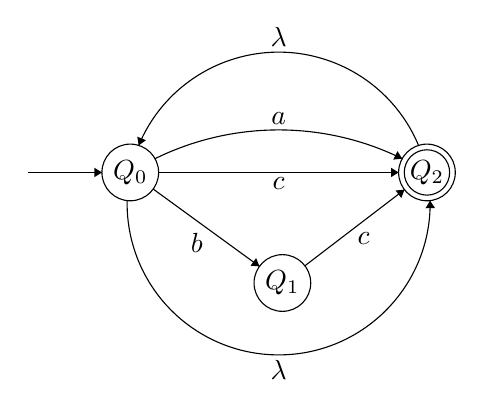
\begin{tikzpicture}[scale=0.12]
            \tikzstyle{every node}+=[inner sep=0pt]
            \draw [black] (22,-25.4) circle (3);
            \draw (22,-25.4) node {$Q_0$};
            \draw [black] (53.4,-25.4) circle (3);
            \draw (53.4,-25.4) node {$Q_2$};
            \draw [black] (53.4,-25.4) circle (2.4);
            \draw [black] (38.1,-37.1) circle (3);
            \draw (38.1,-37.1) node {$Q_1$};
            \draw [black] (11.2,-25.4) -- (19,-25.4);
            \fill [black] (19,-25.4) -- (18.2,-24.9) -- (18.2,-25.9);
            \draw [black] (24.62,-23.942) arc (116.20086:63.79914:29.625);
            \fill [black] (50.78,-23.94) -- (50.28,-23.14) -- (49.84,-24.04);
            \draw (37.7,-20.4) node [above] {$a$};
            \draw [black] (53.735,-28.377) arc (1.05856:-181.05856:16.038);
            \fill [black] (53.73,-28.38) -- (53.25,-29.19) -- (54.25,-29.17);
            \draw (37.7,-45.21) node [below] {$\lambda$};
            \draw [black] (24.43,-27.16) -- (35.67,-35.34);
            \fill [black] (35.67,-35.34) -- (35.32,-34.46) -- (34.73,-35.27);
            \draw (29.05,-31.75) node [below] {$b$};
            \draw [black] (40.48,-35.28) -- (51.02,-27.22);
            \fill [black] (51.02,-27.22) -- (50.08,-27.31) -- (50.69,-28.11);
            \draw (46.7,-31.75) node [below] {$c$};
            \draw [black] (25,-25.4) -- (50.4,-25.4);
            \fill [black] (50.4,-25.4) -- (49.6,-24.9) -- (49.6,-25.9);
            \draw (37.7,-25.9) node [below] {$c$};
            \draw [black] (22.89,-22.539) arc (157.36907:22.63093:16.046);
            \fill [black] (22.89,-22.54) -- (23.66,-21.99) -- (22.74,-21.61);
            \draw (37.7,-12.17) node [above] {$\lambda$};
        \end{tikzpicture}
    \end{center}
\end{frame}

\begin{frame}[t]{Converting a right-linear grammar to an FA}
    Let $G = (V, T, S, P)$ be a right-linear grammar. We want to create an FA $M = (Q, \Sigma, \delta, q_0, F)$ such that $L(M) = L(G)$. Sketch of the procedure:
\end{frame}


\begin{frame}{Exercise}
    \textbf{Exercise.} Convert the following right-linear grammar to an equivalent FA.
    \begin{align*}
        S & \rightarrow aA|a|cC|c|bB|b \\
        A & \rightarrow aA|a|bB|b      \\
        B & \rightarrow bB|b           \\
        C & \rightarrow cC|c|bB|b
    \end{align*}
\end{frame}


\begin{frame}{Equivalence between regular grammars and FAs}
    \textbf{Theorem.} Every regular language has a regular grammar that generates it and every regular grammar generates a regular language.\footnote{This theorem assumes a result about the relation between right-linear and left-linear grammars. Do you see what it is?}
\end{frame}


\end{document}